\section{Auswertung des Textanteils der Kurseinheiten}
Bei der Auswertung des Textanteils der Kurseinheiten, werden die verfügbaren PDF-Dokumente des Autors analysiert. Im ersten Schritt werden aus den PDF-Dokumenten alle Leerseiten, das eventuell enthaltene Glossar, alle Verzeichnisse und sonstige nicht zum eigentlichen Kurstext gehörende Inhalte entfernt. Auch Kurseinheiten, welche nur ein Glossar oder ähnliches darstellen werden nicht berücksichtigt. Danach wird für jeden Kurs eine Seite mit möglichst großem Textanteil gesucht. Darauf wird anhand dieser Kennzahl ein nach der Anzahl der Kurseinheiten der Kurse gewichtete Durchschnitt gebildet. Somit ergibt sich ein durchschnittlicher Wert für eine Seite welche möglichst vollständig mit Text bedeckt ist. Dieses vorgehen soll Unterschiede in Schriftgröße und verwendeter Seitenfläche ausgleichen.
Daraufhin werden alle vorliegenden bereinigten Kurseinheiten mittels des Tools \textit{PDF-Analyzer 5.0}\footnote{http://www.is-soft.de} analysiert. Die Ergebnisse sind der Abbildung \ref{fig:AuswertungKurseinheiten} zu entnehmen. Danach wird die ermittelte Anzahl an Wörter mit der Anzahl der Seiten ins Verhältnis gesetzt.

\begin{sidewaysfigure}
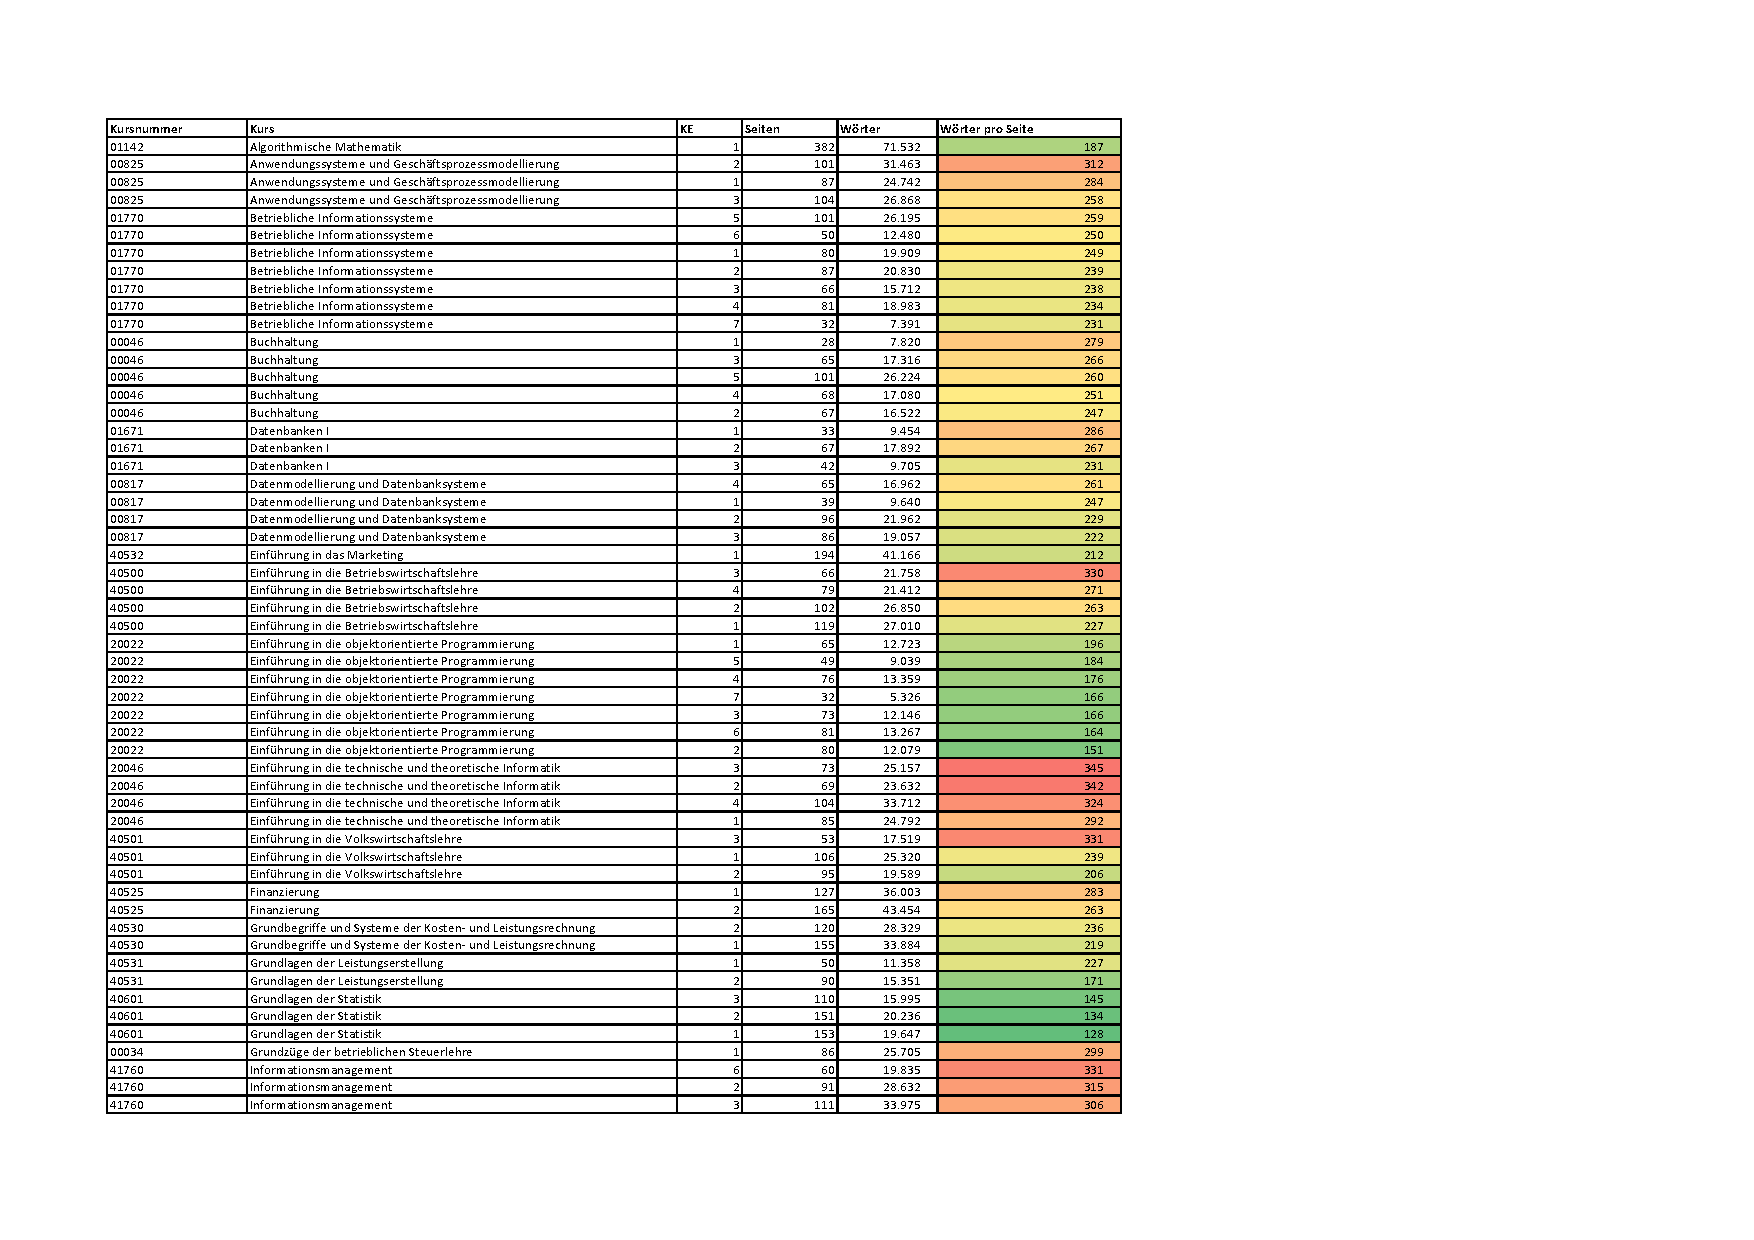
\includegraphics[width=0.95\textwidth,center]{AnalyseKurseinheiten.pdf}
\caption{\label{fig:AuswertungKurseinheiten}Analyse der Kurseinheiten}
\end{sidewaysfigure}

\todo[inline]{Es wird nur eine Seite des PDFs angezeigt}

Bei dieser Analyse sind folgende Punkte zu berücksichtigen, welche die Auswertung verfälschen können:
\begin{itemize}
\item Es werden auch Buchstaben als Wörter gewertet (beispielsweise in Formeln oder Code)
\item Nicht jede Seite einer Kurseinheit wird vollständig genutzt
\item Nicht jede Fläche, die nicht durch Text in Anspruch genommen wird, enthält automatisch einen anderen visuellen Inhalt
\end{itemize}

\section{Auswertung Moodle-Beteiligung}

\begin{sidewaysfigure}
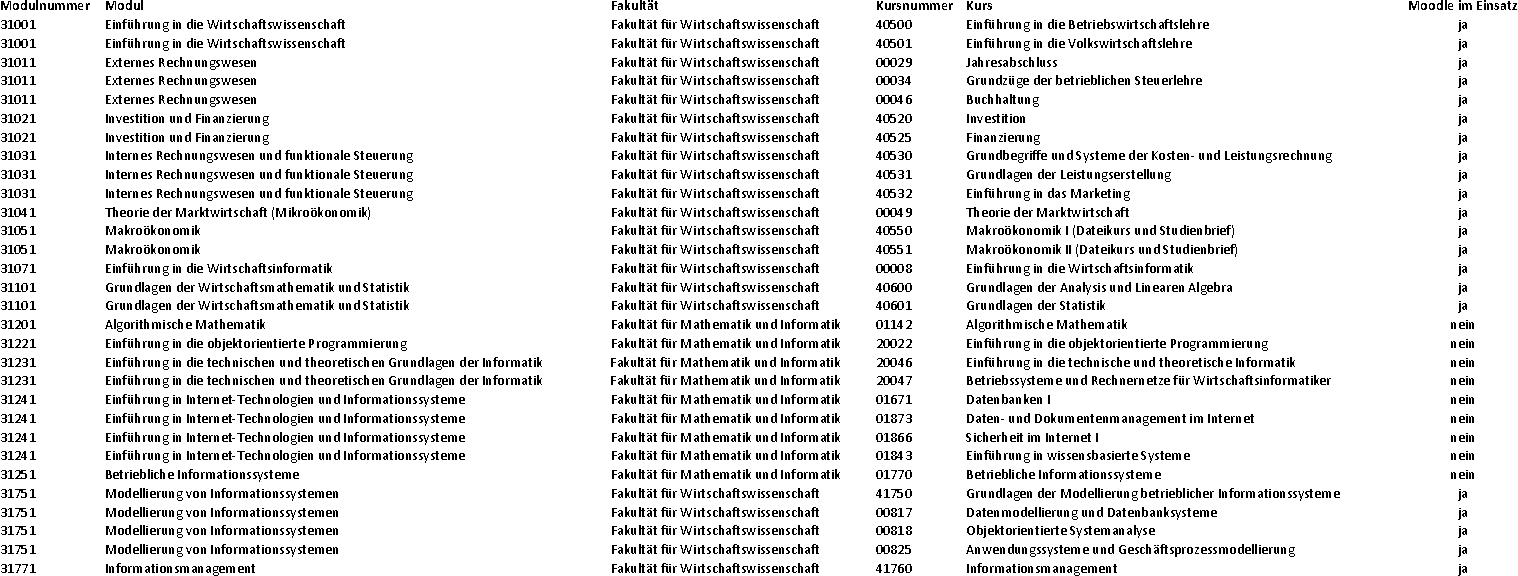
\includegraphics[width=0.95\textwidth,center]{VerwendungMoodleZuschnitt.pdf}
\caption{\label{fig:VerwendungMoodle}Verwendung von Moodle in den Pflichtmodulen des Bachelorstudiengangs Wirtschaftsinformatik (Sommersemester 2018)}
\end{sidewaysfigure}